This section aims to provide a comprehensive list of keywords and their corresponding definitions and uses in the context of the Script Assembler. 

\section{Options}

Options are one of the two types of keywords that can be used within a script. They are used to set specific parameters or configurations for the specific script execution, essentially acting as flags that modify certain behaviors when dealing with the script. It doesn't require a value to be assigned to it, so its presence alone is enough to trigger the intended effect. The position of the option keyword within the script is not crucial, so it can be placed anywhere within the script while keeping its intended effect intact.

During the making of the project, one option keyword has been implemented: 

\subsection{Option: NO\_KETOP}

The NO\_KETOP option keyword can be used by typing the following line anywhere within the script:

\begin{verbatim}
    @NO_KETOP
\end{verbatim}

If this option keyword is present, the "no\_ketop" flag will be set for the entire script. This ensures that certain components that check if a KeTop device is connected are disabled, allowing the script to run without the prerequisite of a KeTop device. This is most useful for specific test scripts that have to be run without a KeTop, like installation scripts. 

\section{Modifiers}

Modifiers are the second type of keywords that can be used within a test script. They differ from options in that they require a body, specified by the presence of indentation, to function properly. The body of a modifier contains further lines of the test script, the modifier keyword itself defines under what conditions the body should be included in the final script. Generally speaking, modifiers are used to either conditionally include or exclude certain parts of the script, or set them in a specific order. 

Bodies of modifiers can also contain other modifiers, allowing the creation of complex and more specific test scripts. 

During the making of the project, the following modifier keywords have been implemented:

\begin{itemize}
    \item VERSION
    \item OS
    \item BRACKETSTART and BRACKETEND
    \item PREAMBLE
\end{itemize}

\subsection{Modifier: VERSION}

The VERSION modifier keyword can be used following the syntax:

\begin{verbatim}
    @VERSION <component> <comparison> <version>
        <body>
\end{verbatim}

Where:
\begin{itemize}
    \item \textbf{<component>} is the label of the component that is being checked, for example "BIOS".
    \item \textbf{<comparison>} is a comparison operator, such as ">", "<", ">=", "<=", "==" or "!=".
    \item \textbf{<version>} is the version of the component that the test script is being run on, in the format of "X.Y.Z" where X, Y and Z are integers.
\end{itemize}

If the version modifier keyword is present, the body of the modifier will only be included in the final script if the condition concerning the component version is met. This allows for the creation of test scripts that behave differently based on the component version of the device. 

\subsection{Modifier: OS}

The OS modifier keyword can be used following the syntax:

\begin{verbatim}
    @OS <os>
        <body>
\end{verbatim}

Where:
\begin{itemize}
    \item \textbf{<os>} is the label of the operating system that is being checked, for example "WIN10".
\end{itemize}

If the OS modifier keyword is present, the body of the modifier will only be included in the final script if the device's operating system matches the specified system. 

\subsection{Modifier: BRACKETSTART and BRACKETEND}

The BRACKETSTART and BRACKETEND modifier keywords do not require any parameters, only the keyword itself and its body:

\begin{verbatim}
    @BRACKETSTART
        <body>

    @BRACKETEND
        <body>
\end{verbatim}

If a script containing a BRACKETSTART or BRACKETEND modifier keyword is being run together with other test scripts, the body of these modifiers will be run before and after the content of all other test scripts respectively. If a batch of test scripts contains multiple scripts containing these modifiers, the bodies of the modifiers will be run in the order they appear in the batch, meaning that the body of the first BRACKETSTART modifier will be run before the body of the second BRACKETSTART modifier. The same principle applies to the BRACKETEND modifiers.

Therefore, these modifiers can be used to set up tests that require a certain amount of time to have passed, before the result can be observed. For example, if a test script is meant to check the behavior of a device after it has been active for 30 minutes, the BRACKETSTART modifier can be used to set up the test, and the BRACKETEND modifier can be used to check the results after the 30 minutes have passed. In the meantime, other test scripts can be run between the two "bracket tests", allowing for a more efficient use of time when running a batch of test scripts.

\subsection{Modifier: PREAMBLE}

The PREAMBLE modifier keyword can be used following the syntax:

\begin{verbatim}
    @PREAMBLE <index>
        <body>
\end{verbatim}

Where:
\begin{itemize}
    \item \textbf{<index>} is an integer that specifies the order in which the preambles are run, with 1 being the first preamble to be run.
\end{itemize}

When one or multiple test scripts containing a PREAMBLE modifier keyword is being run together with other test scripts, the body of the PREAMBLE keyword will be run before the content of all other test scripts, including lines in the body of a BRACKETSTART modifier. In the case of multiple PREAMBLE modifiers being present in the batch of test scripts, the bodies will be run in the order of their specified index.

The PREAMBLE modifier can be used to write scripts that test certain installation processes and their successful completion before the rest of the test scripts are run.

\section{Visual Example}

Consider the following diagram:

\begin{figure}[ht]
    \centering
    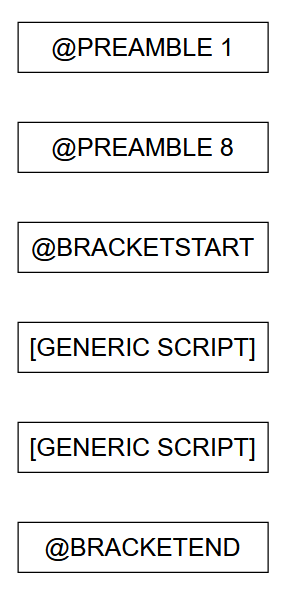
\includegraphics[width=0.35\textwidth]{pics/script-order.png}
    \caption{Simple Diagram depicting the order scripts with a certain modifier keyword are run in.}
    \label{fig:script-order}
\end{figure}

Here, it can be seen how some specific test scripts are arranged in the final script.

\begin{enumerate}
    \item The bodies of the PREAMBLE modifiers are ordered first if present. In the case of multiple PREAMBLE scripts being present, the specified index is used to order them accordingly. As seen in the diagram, leaving out certain indices doesn't lead to any issues, the ordering occurs as intended.
    
    \item The bodies of the BRACKETSTART modifiers are ordered next if present. In the case of multiple BRACKETSTART scripts being present, the order they appear in the batch is maintained.
    
    \item At this point, the content of all test scripts not containing any order-modifying keywords are placed. Their order is determined by the order they appear in the batch.
    
    \item Lastly, the bodies of the BRACKETEND modifiers are ordered if present. In the case of multiple BRACKETEND scripts being present, they follow the same principle as the BRACKETSTART modifiers, meaning that the order they appear in the batch is maintained.
\end{enumerate}